\section{Suppress the Spiders using FFT}
\label{sec:suppression}
We now want to use the knowledge we have gained about the Fourier transformation of different features, especially of features which resemble spiders, to suppress the signal of the spiders. The idea is to manipulate the Fourier transform of the data and then transform the result back via the inverse Fourier transformation.\\
We take the data from HD142527, warp it to the $r$-$\varphi$ plane and correct for the radial intensity drop. For the transformation we choose the radius range as in figure \ref{fig:warped_254_454} namely: $R=254-454$, such that the object we want to look at is placed in the center. In order to make sure that the aperture flux of other objects than the spiders, mainly point sources like exoplanets, is conserved we will use the ghost at radius $323$ as a reference. The ghost is not perfectly in the center of the radius range, but this is not important for our purpose. The only thing which will happen, is that the aperture flux will change a bit when warping the image to the $r$-$\varphi$ plane.\\
Figure \ref{fig:rad0} shows the Fourier transform of the warped and flattened image at different radial frequencies. In contrast to the Fourier transform of the simulated spiders, the signal is not Gaussian anymore, since there are other features on top, like the ghost and the noise.
\begin{figure}[H]
	\centering
		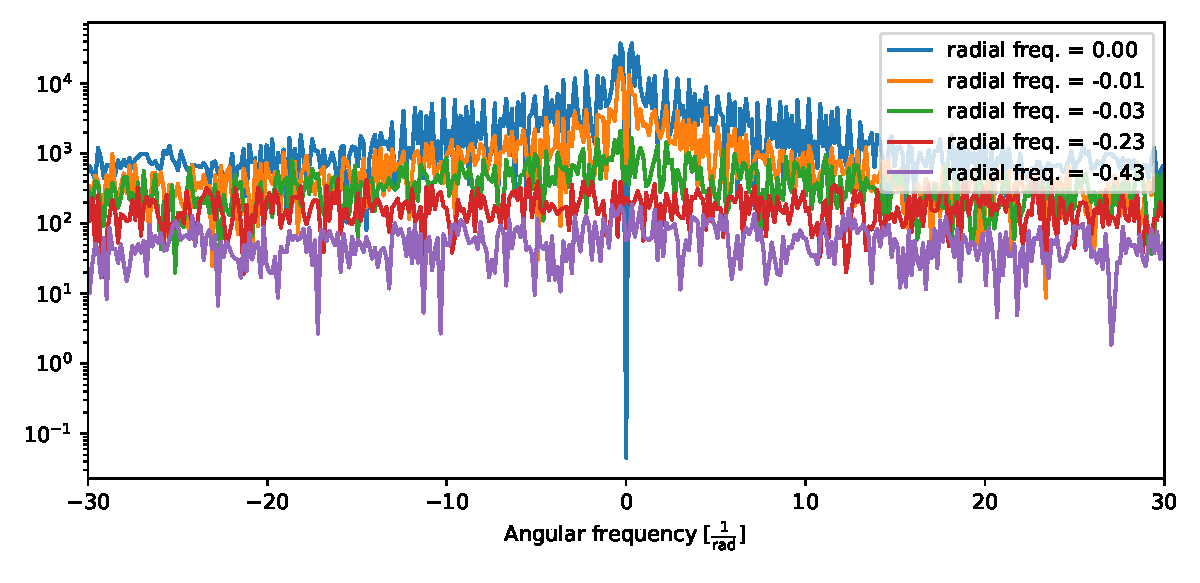
\includegraphics[width=1.0\textwidth]{pics/rad0.pdf}
		\caption{Several horizontal cuts through the frequency plane of the image data shown in figure \ref{fig:HDsuppcentralfreq_R254_R454_-0.5to0.5}(a).}
		\label{fig:rad0}
\end{figure} 

\subsection{High Frequencies}
As we saw in section \ref{sec:pointlike} the angular range in which a point-source, Gaussian or PSF, will produce a significant frequency signal is within $[-50, 50] \frac{1}{\mathrm{rad}}$ and the radial range is within $[-0.2, 0.2] \frac{1}{\mathrm{px}}$. When we consider the noise, the range is even smaller as we saw in section \ref{sec:noise}.  
Therefore we first thought it would be a good idea to suppress everything which is outside of this area by a factor of $1000$. However it turned out that this is not the best idea, since the high frequencies are responsible for the edges in the image. By suppressing the high frequencies we would therefore blurry the image. This might not look like being a problem, since due to the noise the image is already blurred. As long as the point-source we look at is sufficiently large and bright this is indeed no problem, but as soon as the point-source gets fainter and smaller, it starts to disappear due to the blurring. Since we are more interested in objects of the second kind it is no option to suppress the high frequencies. Also we would not gain any positive effect through this suppression.\\
We also need to keep in mind here that we are plotting the absolute values of the frequency space and thus ignore big parts of the phase information as well as negative values. But we should not ignore this fact, when we do the suppression.\\
An other attempt tried was to subtract the mean of the noisy frequency background from the whole frequency space, but this was an even worse idea. Due to the subtraction the whole back transformed image gets a weaker intensity. All structures stay unchanged, but are weaker. Like this it would be even harder to find faint structures, especially if they come too close to the numerical limits. 

\subsection{Subtraction}
\label{sec:suppression_subtraction}
In order to be able to suppress the spiders, we need to understand them. As we learned in section \ref{sec:fourier} the spiders itself can be created by a convolution of the image containing the position and separation information, this means one pixel thick lines at the position of the spiders, and the image of a spider which contains the shape information, as the intensity and the width.\\
The spiders are added on top of the image. So the only option to suppress them completely is to subtract them, which is due to the linearity of the Fourier transformation also a subtraction in the frequency space. If we would do a division in the frequency space instead, which corresponds to unfolding the convolution. We would still remain with some parts of the information and maybe destroy image information, because the spiders are the result of first a convolution and then an addition.  This means we need to subtract the signal in the frequency plane generated by the spiders.\\
Since we do a subtraction we cannot only look at the absolute frequency values, we need to consider the complete real part. This means that we cannot ignore the position information of the spiders, which makes it a lot more complicated. Already now we can say that suppressing the spiders by subtracting certain frequencies in the Fourier space is a bad idea. Due to the fact that the point sources and the spiders are both located at the central frequencies we need to know exactly how the frequency signal produced by the spiders looks like. As we saw in \ref{sec:Fourier_spiders} this signal is complex and depends on the separations, the positions, the intensities and the widths of the spiders. We need to know all these parameters in order to be able to subtract the right frequencies. However if we know all these parameters precisely we can also subtract the spiders in the image plane and do not have to go to the frequency plane. Although we already know that it is not a good idea, we will still try it out. \\
\begin{figure}[H]
	\centering
		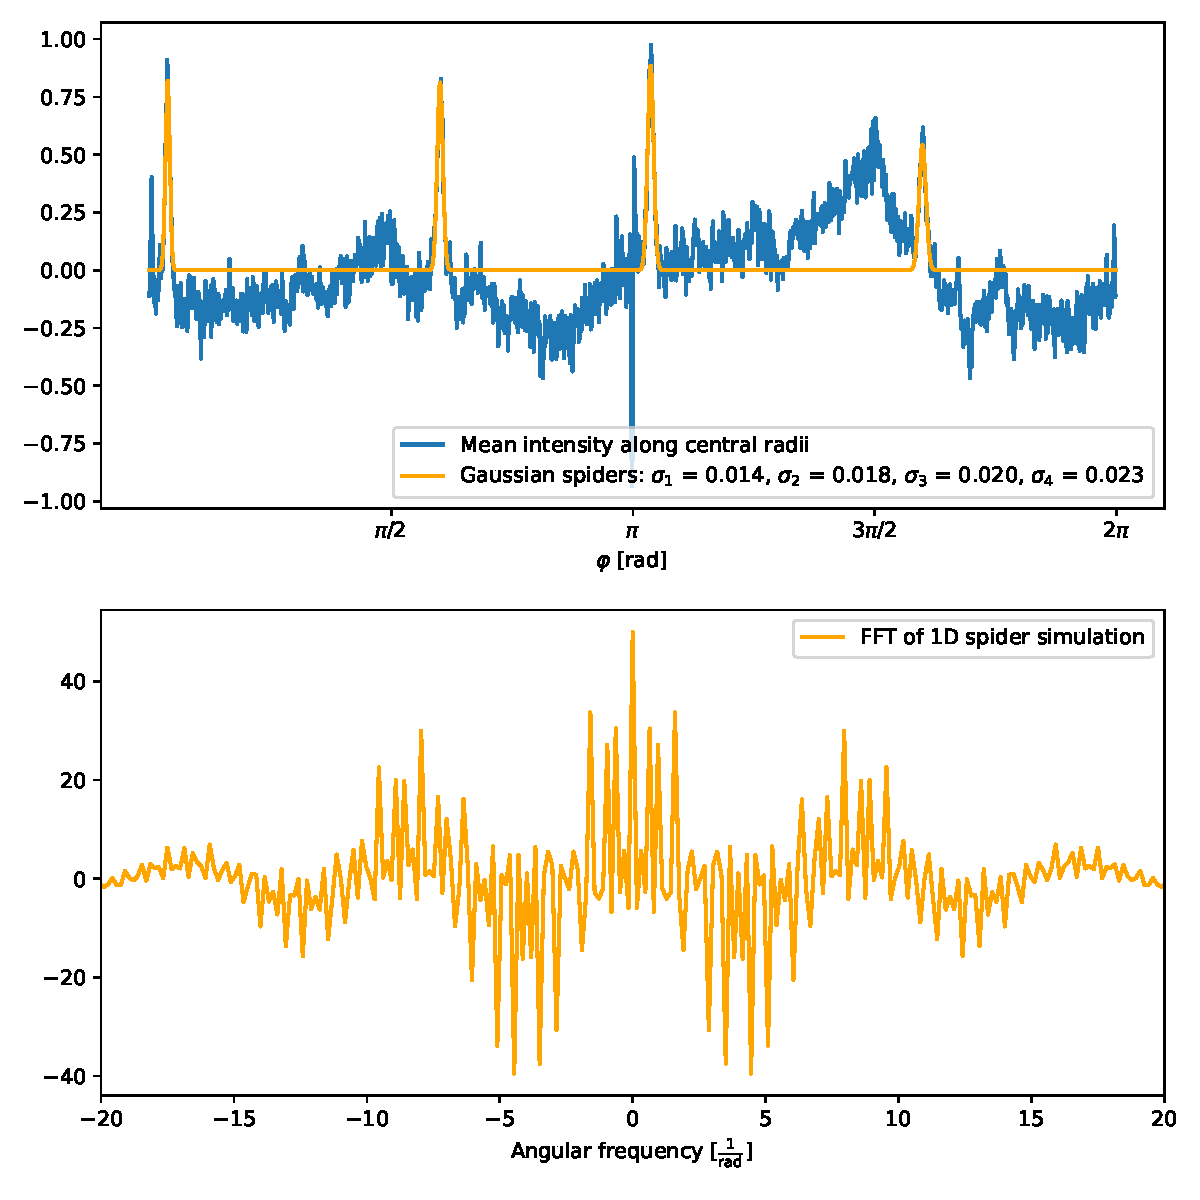
\includegraphics[width=1.0\textwidth]{pics/Spider_Gaussianfit_FFT.pdf}
		\caption{We fit Gaussian profiles to the mean intensity of the spiders in the central radial range (top). The function resulting from the fits is Fourier transformed (bottom).}
		\label{fig:Spider_Gaussianfit_FFT}
\end{figure}
To find the frequency spectrum which we have to subtract from the central radial frequency, which is the most important one (see section \ref{sec:fourier}), we sum up the central radial frequencies and fit Gaussian profiles to the spiders, see figure \ref{fig:Spider_Gaussianfit_FFT}. The Fourier transformation of the 1 dimensional fit has the same shape as the Fourier transformation of the spiders for radial frequency zero, the only difference is the intensity. We know that the central frequency is equal to the total intensity of the image, we therefore sum up the total intensity of the spiders only and use this information to adapt the intensity of the simulated Fourier transform. Then we subtract it from the frequency space of the data. The resulting frequency space and its back-transformed image are shown in figure \ref{fig:HDsubtraction}(b). To get back into the $r$-$\varphi$ plane we use the inverse Fourier transformation. Figure \ref{fig:HDsubtraction}(a) shows the warped and flattened image from $R=254-454$ and its Fourier transform. \\
When comparing the image before and after the subtraction, we see that around the central radial range the spiders have almost completely vanished. However we need to keep in mind that this was only possible by fitting Gaussian profiles to the spiders and if an object is really close to a spider it will be subtracted away, because the fit will count it to the spider. \\
From the steps we have made so far the aperture flux increases by $0.67$ \% compared to the initial aperture flux for ghost 2. We also insert a PSF close to the spider, where ghost 2 is, but in the central radius. If we place the PSF inside the spider it vanishes due to the subtraction, but if we place it next to the spider its aperture flux increases by $278$ \% for the PSF, here we use a PSF which is approximately $10^{-6}$ times less bright then the star. 
\begin{figure}[H]
	\centering
		\subfigure[]{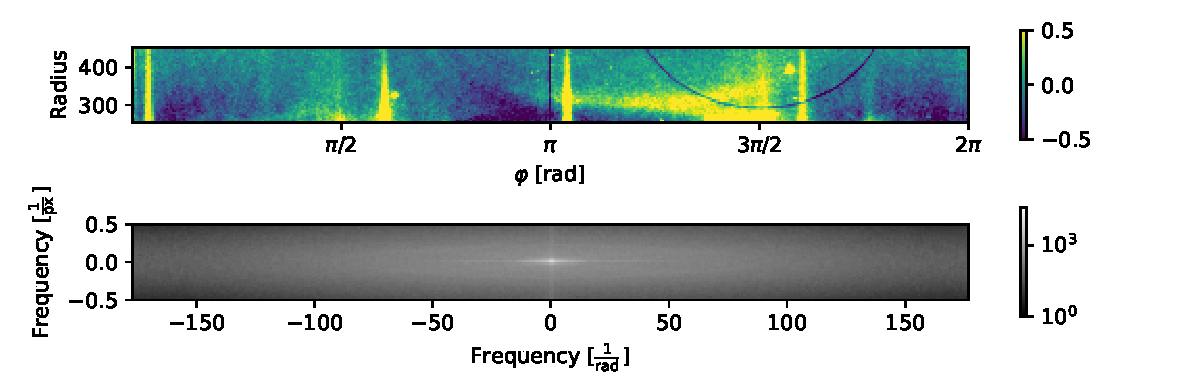
\includegraphics[width=1.1\textwidth]{pics/HDflatten_R254_R454_-0.5to0.5.pdf}}
		\subfigure[]{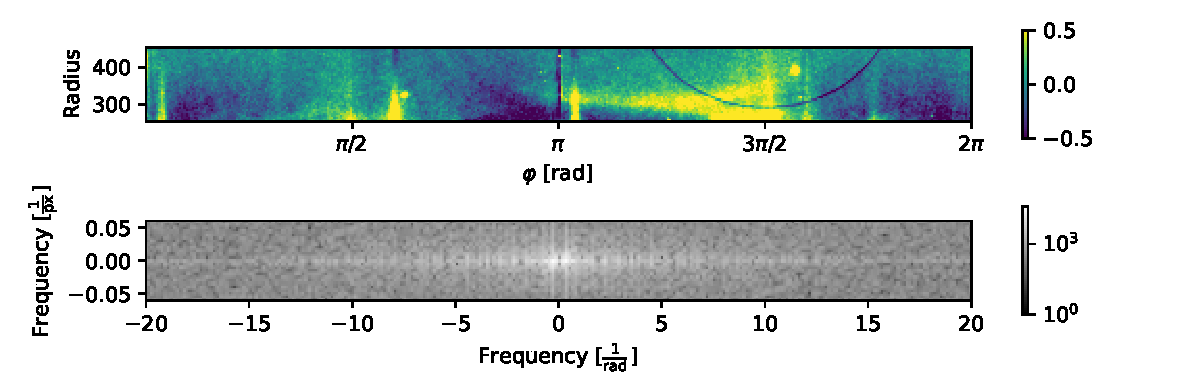
\includegraphics[width=1.1\textwidth]{pics/HDsubtracted.pdf}}
\caption{An image from HD142527 which has been warped to the $r$-$\varphi$ plane and flattened and its Fourier transform (a). After a subtraction of a specific pattern at radial frequency zero, the spiders around the central radius are almost completely vanished(b).}
\label{fig:HDsubtraction}
\end{figure}

\subsection{Division}
\label{sec:suppression_division}
At the beginning of this work we accidentally did a division in the frequency space instead of a subtraction and we only realized this mistake at the very end of the thesis. As we already discussed in section \ref{sec:suppression_subtraction} division is not the right way to completely suppress the spider. Still we can achieve that the spiders become really narrow and less bright through a division in the frequency space. The only problem is that we also change the rest of the image data and not only regions around the spiders. Depending on how large this change is, the possibility of dividing could still be a good option. The division has the advantage that it is a lot more stable, meaning that we do not need to know the exact shapes and intensities of the spiders. Additionally we do not need to know the position information, since we do not change the sign by dividing by a positive number. \\

\subsubsection{Suppress Central Radial Frequencies}
\label{sec:sup_cen_radialfreq}
From our investigation of the Fourier transformation for spider-like structures, we found that their most important features are where the radial frequency is zero. Therefore, we first want to suppress the frequencies, which are caused by the spiders, at radial frequency zero.\\
As we saw in section \ref{sec:gaussian} the spiders produce a signal in the frequency plane, which is close to a Gaussian, this is especially the case when the radial frequency is equal to zero. We divide our central radial frequency by the Gaussian profile with width $\sigma = 8.7 \frac{1}{\mathrm{rad}}$, which we found from our simulations of the spiders, see figure \ref{fig:simspi_noise_angularfreq}. By doing this we ignore the fact that we have some oscillations on top of the true signal. But this is totally fine, since we only aim to transform the spiders into faint lines and the oscillations contain the separation information between the different spiders, which we will not need. Still we reassure that this approximation is appropriate by comparing the resulting back-transformed images after a division by the Gaussian profile and after a division by the Fourier transform at radial frequency zero which we get from our simulations. From the comparison we find that the Gaussian profile is a really good approximation, since by eye we cannot see any differences between the resulting back-transformed images and also the aperture fluxes of the ghosts are almost the same. We also compute the aperture flux of a PSF which we place on the image far away from the spiders and also this aperture flux is almost the same, also for different intensities of the PSF.\\
As a next step we want to find out in which angular range around the central frequency we need to divide by the Gaussian. This is a really important parameter because, if the angular width is so large, that the value of the Gaussian profile at this position is smaller than one, the division will lead to an increase of the intensity instead of a suppression. Figure \ref{fig:rad0_diffsubwidths} shows the aperture flux of the ghost after the division by a Gaussian at radial frequency zero for different angular frequency ranges around zero. The orange line marks the aperture flux of the ghost after the warping and the correction for the radial drop-off, we call it the initial aperture flux. Whereas the blue dots mark the aperture flux of the ghost after the division by the Gaussian for different angular widths.\\
Since it is an advantage, if the aperture flux increases through the procedure, we choose the width with which we get the largest aperture flux, which is the case for $9.1 \frac{1}{\mathrm{rad}}$. This means we divide by the Gaussian in the following angular range: $[-9.1, 9.1] \frac{1}{\mathrm{rad}}$.\\
An increase of the aperture flux is really good, because it means that the spiders are being suppressed without suppressing the ghost. Ghost 2, at which we are looking, is a good indicator for this, because in this image it is situated close to a spider.
\begin{figure}[H]
	\centering
		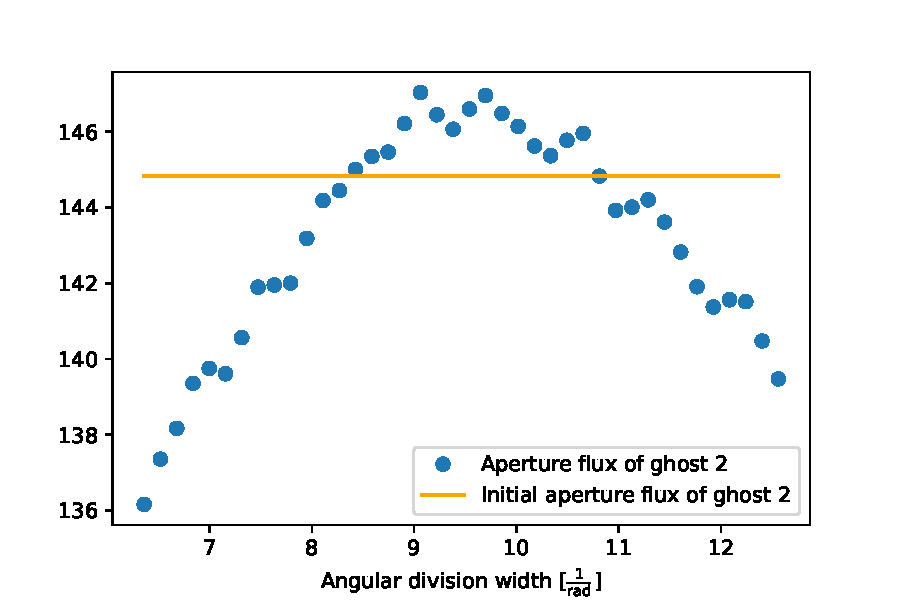
\includegraphics[width=1.0\textwidth]{pics/rad0_diffsubwidths.pdf}
		\caption{For radial frequency zero the Fourier transform of the image data is divided by a Gaussian which has its center at angular frequency zero. The division is not performed along the complete angular range, but only for a certain width around zero. We have plotted the aperture flux of ghost 2 for different angular division widths. The width which produces the largest flux is ideal.}
		\label{fig:rad0_diffsubwidths}
\end{figure}
Other parameters in this suppression are the intensity and the width of the Gaussian profile. We find that the resulting back-transformed image is not at all sensible on this variables. This is due to the fact that we divide by the Gaussian and do not subtract it. An other reason for the insensibility on the width of the Gaussian profile is that we only look at a narrow angular range, where the width of the Gaussian profile does not have a big influence. \\
Figure \ref{fig:HDsubtraction}(a) shows the warped and flattened image from $R=254-454$ and its Fourier transform. In figure \ref{fig:HDsuppcentralfreq_R254_R454_-0.5to0.5} the Fourier transform which is divided by the Gaussian profile at radial frequency zero in the above defined angular range and its back-transformed image are shown. To get back into the $r$-$\varphi$ plane we use the inverse Fourier transformation. When we compare the image before and after the Gaussian division we can already observe that the spiders are a lot less bright. Especially around the central radius the results are good. This region is the most important for us, since it is the only region, where the warping does not change the shape of the objects. Below the central radius the spiders almost stay the same or change only slightly and above the central radius we have a trend to the other extreme, meaning we have negative values. We also observe that the noise gets weaker and is smoother distributed.\\
From the steps we have made so far the aperture flux increases by $6.64$ \% compared to the initial aperture flux for ghost 2 and by $49.73$ \% for the PSF, here we use a PSF which is approximately $10^{-6}$ times less bright then the star. 
\begin{figure}[H]
	\centering
		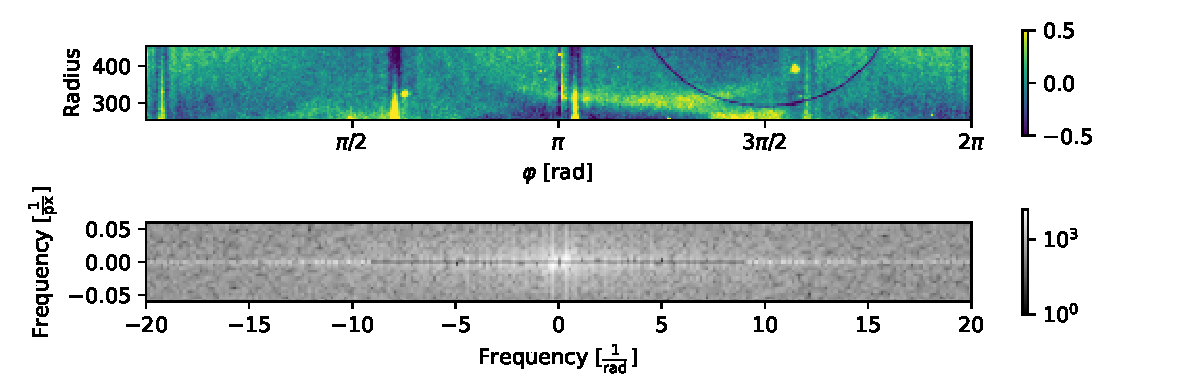
\includegraphics[width=1.1\textwidth]{pics/HDsupprcentralfreq_R254_R454_-0.5to0.5.pdf}
		\caption{An image from HD142527 which has been warped to the $r$-$\varphi$ plane and flattened and its Fourier transform (a). After a division of the central frequencies at radial frequency zero by a Gaussian profile, the spider in the back-transformed image are less bright (b).}
\label{fig:HDsuppcentralfreq_R254_R454_-0.5to0.5}
\end{figure}

\subsubsection{Suppress Low Frequencies}
As we saw during the simulation of the spiders, not only the frequencies at radial frequency zero have non-zero values, but there is also an extension into the radial frequencies with non-zero values. In the following we will also suppress the frequencies which are caused by the spiders in this regime by using division. But due to the noise level, the interesting radial regime only goes until approximately $[-0.06, 0.06] \frac{1}{\mathrm{px}}$. As we already discussed in section \ref{sec:sup_cen_radialfreq} the regime is even smaller, since we need to avoid to divide through values which are smaller than one. The same holds for the angular range. The angular range is smaller for larger absolute radial frequency values, since the intensity of the complete signal is overall smaller. In conclusion we will only be able to suppress the lowest frequencies.\\
First of all we have to choose a Gaussian profile with an adequate width and intensity. As before when we suppressed the central radial frequency, we choose the Gaussian profiles such that it best fits to the signal of our spider simulation. For the signal at radial frequency $-0.005$/$0.005 \frac{1}{\mathrm{px}}$ (these are the ones closest to the radial frequency center and they are the same due to the symmetry of the Fourier transform) we choose a Gaussian profile with width $\sigma_s = 6.4 \frac{1}{\mathrm{rad}}$ and intensity $I_s = 0.84 I = 8.4 \cdot 10^3$ where $I$ is the intensity of the Gaussian profile used for suppressing the frequencies at radius zero. As before in section \ref{sec:sup_cen_radialfreq} the width and the intensity of the Gaussian profile are not so important for the suppression and it does not matter if they differ a bit. But the angular frequency width $w_s$ in which we do the division (as in section \ref{sec:sup_cen_radialfreq}) as well as the radial frequency width $h$ is essential.\\
To find these two parameters we use the same procedure we used in section \ref{sec:sup_cen_radialfreq} to find the angular frequency width $w$ for radial frequency zero. Namely we try out different parameters and take the one with which we get the largest aperture flux for ghost 2. As before we will also use a second object in form of a PSF which is placed not in the surrounding of one of the spiders, in order to check does not change the background in unwanted way. The PSF is approximately $10^{-7}$ times less bright then the star. We find that $h = 0.01 \frac{1}{\mathrm{px}}$ and $w_s = 7.2 R \frac{1}{\mathrm{rad}}$, where $R$ is the ratio between the mean central radial frequency (considering only low angular frequencies) and the mean radial frequency in which the division is taking place.\\
The parameters for the other radial frequencies with an absolute value which is larger than $0.005 \frac{1}{\mathrm{px}}$, but still smaller than $h$, are derived from the one at absolute radial frequency $0.005 \frac{1}{\mathrm{px}}$. In figure \ref{fig:simspi_angularfreq} we observed that the non-central low radial frequencies all have the same shape, but different intensities. Therefore we choose the same Gaussian profile for all of them and multiply it by factor $R$.\\
Figure \ref{fig:HDsupplowfreq_R254_R454_-0.5to0.5.pdf} shows the image from HD142527 after the suppression of the low frequencies and the suppression of the central radial frequency. We observe that the overall brightness of each spider from figure \ref{fig:HDsuppcentralfreq_R254_R454_-0.5to0.5} to figure \ref{fig:HDsupplowfreq_R254_R454_-0.5to0.5.pdf} has not changed significantly, but the gradient from lower to larger radii which we had in figure \ref{fig:HDsuppcentralfreq_R254_R454_-0.5to0.5} (b) has almost completely vanished. Also the whole image is a lot smoother. This can also be observed in the aperture fluxes. As ghost 2 is placed near a spider and is almost at the center of the radial range, its aperture flux is almost the same as after the suppression of the central radial frequency only and so the aperture flux increased by $6.74$ \% compared to its initial aperture flux, whereas the aperture flux of the PSF increased by $53.12$ \%. 
\begin{figure}[H]
	\centering
		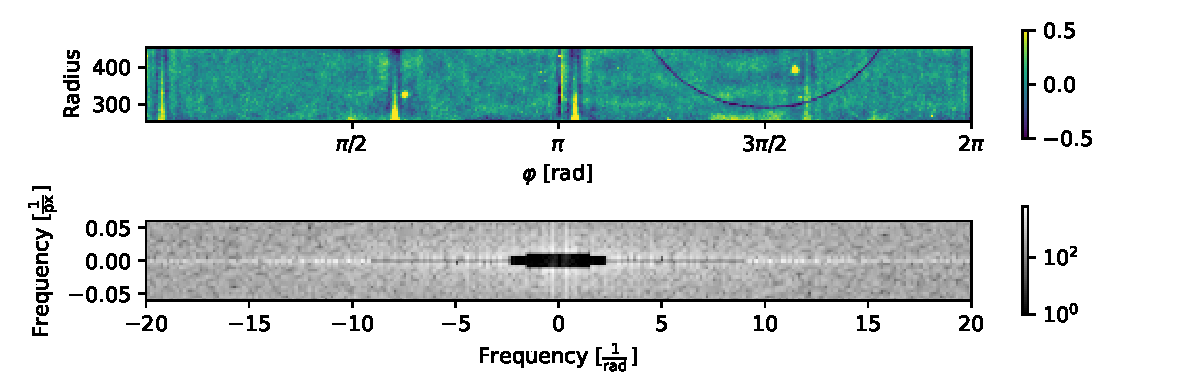
\includegraphics[width=1.1\textwidth]{pics/HDsupplowfreq_R254_R454_-0.5to0.5.pdf}
		\caption{The image from HD142527 after the central radial frequencies and the low frequencies are both suppressed in the frequency plane and transformed back to the image plane via inverse Fourier transformation.}
		\label{fig:HDsupplowfreq_R254_R454_-0.5to0.5.pdf}
\end{figure}
